% Chapter 3
\chapter{Resultados}\label{chap:Results}

Neste capítulo são apresentados os resultados do trabalho desenvolvido,
apresentando a criação do repositório institucional proposto, desde a
sua concepção, \emph{backlog} do produto, protótipos, resultado final
e validação das hipóteses.

\section{Concepção do Repositório Institucional}

A concepção do repositório institucional proposto foi realizada com base
nos desafios e problemas relatados nos trabalhos relacionados, e na análise
dos pontos positivos e negativos encontrados em outros sistemas de repositório
institucional existentes.

Como um dos principais diferenciais do repositório proposto, é que desde o
inicio de seu desenvolvimento ele foi projetado para ser facilmente implantado
e executado em ambientes baseados em nuvem, sendo assim todas as suas configurações
podem ser realizadas por meio de variáveis de ambiente, que em geral podem ser
facilmente definidas pelo próprio painel ou \emph{dashboard} fornecido pelo
provedor de nuvem. A ideia é nunca precisar acessar remotamente a máquina
em que a aplicação está sendo executada para realizar qualquer tipo de configuração.

Outro ponto de diferença é que o repositório proposto somente aceita arquivos no
formato PDF, visando mitigar problemas relacionados a formatação do documento, e
buscando garantir que o usuário ao acessar as publicações, visualize
o documento da mesma forma que o autor originalmente a escreveu. Esta redução
do escopo de formatos de arquivos aceitos pelo repositório, também garante que
todas as publicações estejam normalizadas em um mesmo formato, permitindo a
utilização de técnicas mais especializadas para a extração de texto dos documentos.

Para realizar a escolha do nome e identidade visual do repositório, foram buscados
por termos que remetessem a "Repositório", "Acesso Aberto'' e "Pesquisa", chegando
a escolha do nome RESOAR, uma sigla em inglês para \emph{Research Open Access Repository}.
A sigla "OAR'' que remete a \emph{Open Access Repository} já é baste difundida, e
pode ser encontrada em nomes como o OpenDOAR\footnote{https://v2.sherpa.ac.uk/opendoar/} e
ROARMAP\footnote{https://roarmap.eprints.org/}.

\begin{figure}[H]
    \caption{Identidade visual do repositório}
    \centering
    \frame{
\includegraphics[scale=0.0558]{img/resoar.png}}
    \label{fig:resoar}
    \source{Do próprio autor}
\end{figure}

A Figura \ref{fig:resoar} apresenta a logo ou identidade visual do repositório,
que foi elaborada por um designer contratado da região de Três de Maio - RS,
que desenvolveu tanto a identidade visual quanto os primeiros protótipos do repositório.

Em sua composição é possível perceber um simbolo de lupa embutido na primeira letra "R''
representando a pesquisa. A cor padrão da logo foi escolhida como o laranja com
o código HEX \#ff5400, porem o simbolo também pode ser exibido em outras variações
em preto e branco, escala de cinza ou outras cores.

\section{Backlog do produto}

Nesta seção será apresentado o \emph{backlog} do produto que foi desenvolvido
seguindo a metodologia de \emph{User Stories}, contendo uma lista de funcionalidades
que o sistema final deve conter, além de \emph{mockups} das telas, servindo como uma
base para o desenvolvimento da aplicação.

\begin{table}[H]
    \caption{Tela de Login}
    \begin{tabular}{|p{1cm}|p{14cm}|}
        \hline
        \multicolumn{1}{|c|}{\textbf{01}} & \textbf{Tela de Login}                                                                                                                                                                                                                                                                          \\ \hline
        \multicolumn{2}{|l|}{\begin{tabular}[c]{@{}l@{}}\textbf{Como} usuário do sistema\\ \textbf{Eu quero} realizar o login utilizando meu email e senha\\ \textbf{Para que} possa utilizar as funções presentes no sistema.\end{tabular}}                                                                                                \\ \hline
        \multicolumn{2}{|l|}{\textbf{Critérios de aceitação}}                                                                                                                                                                                                                                                                               \\ \hline
        \multicolumn{2}{|l|}{\begin{tabular}[c]{@{}l@{}}1. Deve possui o botão de exibir/esconder a senha.\\2. Deve possuir os atalhos para as telas de recuperação de senha e cadastro\\ de usuário.\\3. Caso o usuário digitar a senha incorretamente mais de 3 vezes, deve solicitar\\ a resolução de um desafio captcha. \end{tabular}} \\ \hline
        \multicolumn{2}{|c|}{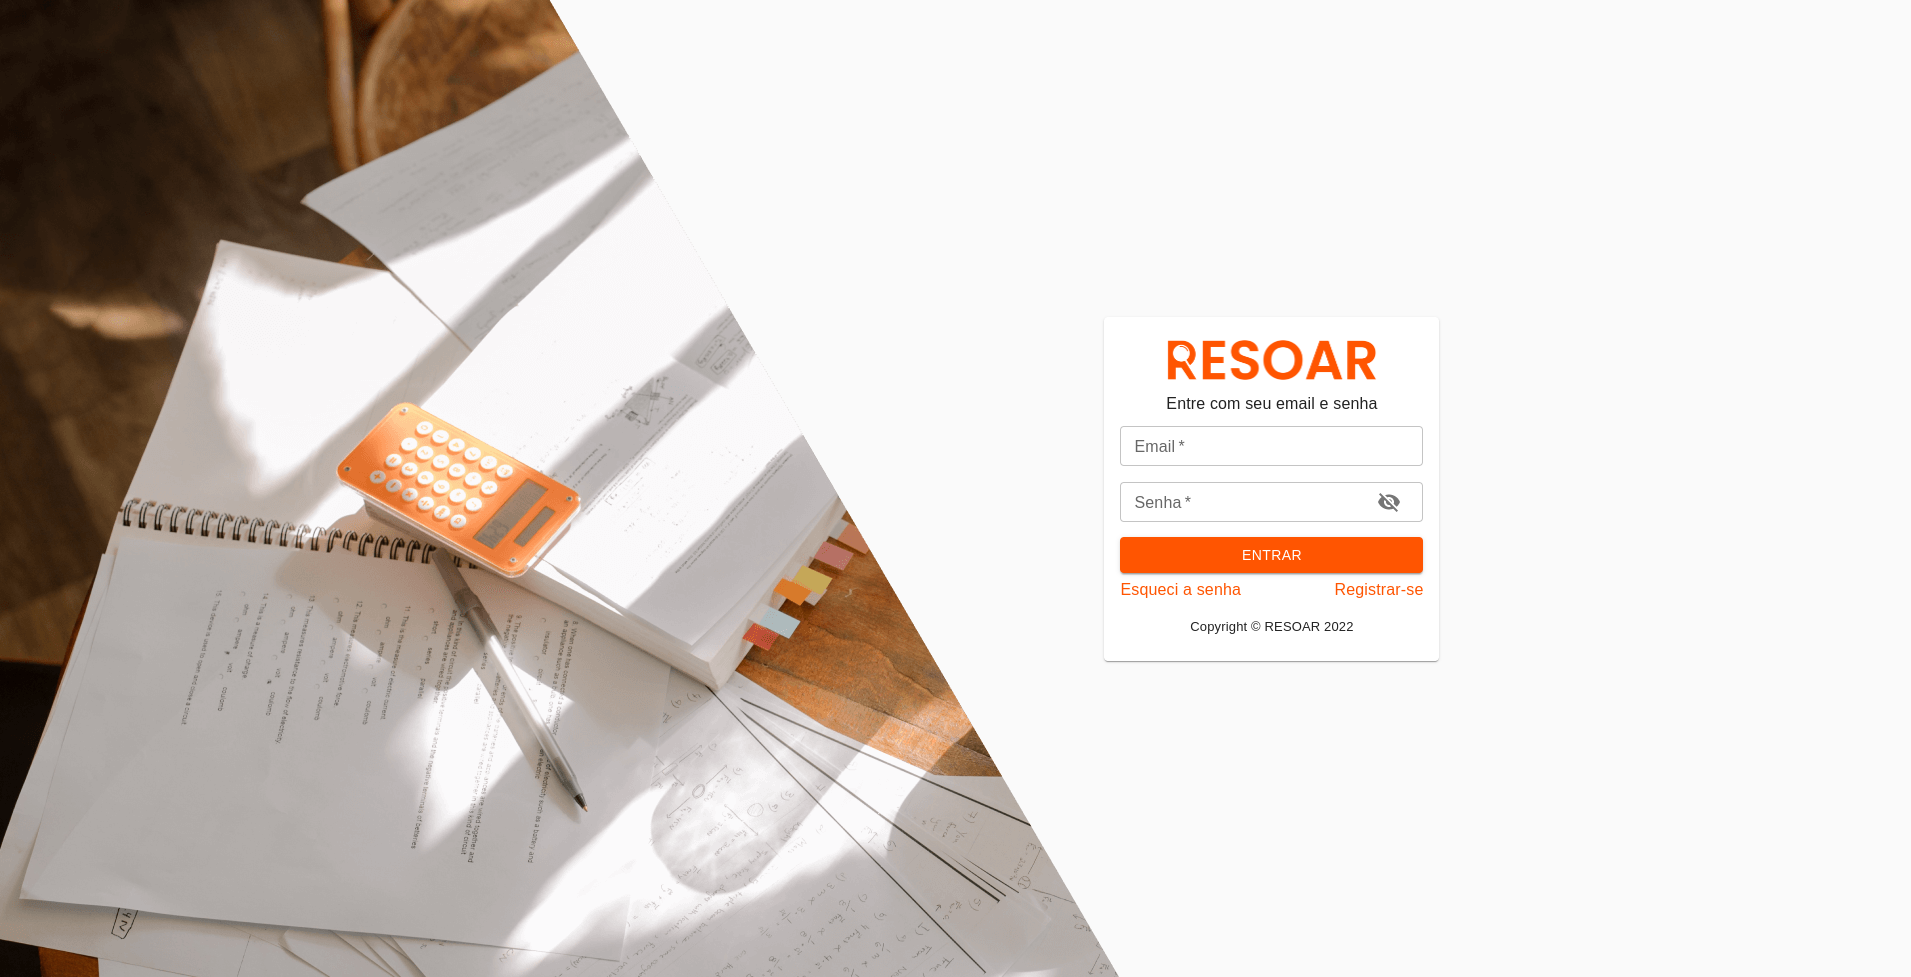
\includegraphics[scale=0.296]{img/resoar-login.png}}                                                                                                                                                                                                                                                           \\ \hline
    \end{tabular}
\end{table}

\begin{table}[H]
    \caption{Cadastro de usuário}
    \begin{tabular}{|p{1cm}|p{14cm}|}
        \hline
        \multicolumn{1}{|c|}{\textbf{02}} & \textbf{Cadastro de usuário}                                                                                                                                                                                   \\ \hline
        \multicolumn{2}{|l|}{\begin{tabular}[c]{@{}l@{}}\textbf{Como} novo usuário\\ \textbf{Eu quero} me cadastrar no sistema\\ \textbf{Para que} possa entrar no sistema.\end{tabular}}                                                                  \\ \hline
        \multicolumn{2}{|l|}{\textbf{Critérios de aceitação}}                                                                                                                                                                                              \\ \hline
        \multicolumn{2}{|l|}{\begin{tabular}[c]{@{}l@{}}1. Deve validar se já existe um usuário cadastrado com o mesmo email.\\2. Deve validar se os dois campos de senha são iguais.\\3. Deve solicitar a resolução de um desafio captcha. \end{tabular}} \\ \hline
        \multicolumn{2}{|c|}{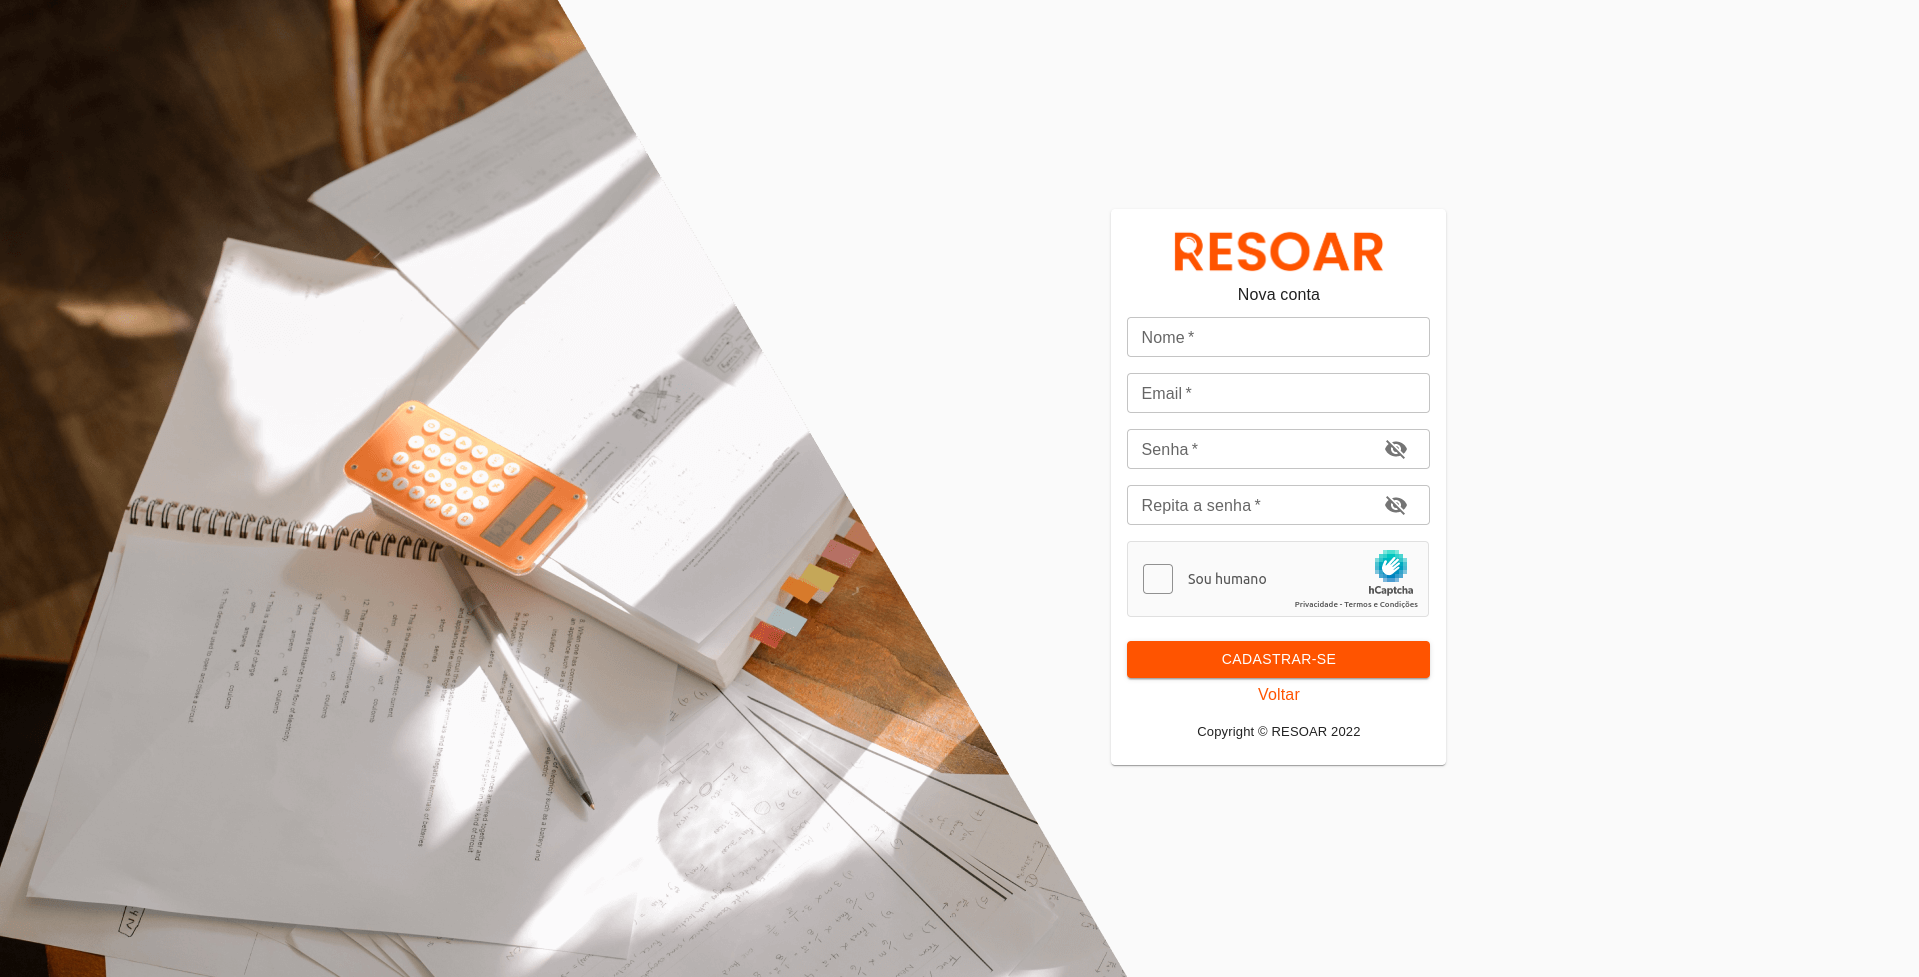
\includegraphics[scale=0.294]{img/resoar-new-account.png}}                                                                                                                                                                    \\ \hline
    \end{tabular}
\end{table}

\begin{table}[H]
    \caption{Recuperação de senha}
    \begin{tabular}{|p{1cm}|p{14cm}|}
        \hline
        \multicolumn{1}{|c|}{\textbf{03}} & \textbf{Recuperação de senha}                                                                                                                                                                                     \\ \hline
        \multicolumn{2}{|l|}{\begin{tabular}[c]{@{}l@{}}\textbf{Como} usuário do sistema\\ \textbf{Eu quero} poder solicitar um email de recuperação de senha\\ \textbf{Para que} possa criar uma nova senha para meu usuário.\end{tabular}}                  \\ \hline
        \multicolumn{2}{|l|}{\textbf{Critérios de aceitação}}                                                                                                                                                                                                 \\ \hline
        \multicolumn{2}{|l|}{\begin{tabular}[c]{@{}l@{}}1. Deve validar se o email informado existe no sistema.\\2. Deve enviar um email de recuperação, com validade máxima de 3 horas.\\3. Deve solicitar a resolução de um desafio captcha. \end{tabular}} \\ \hline
        \multicolumn{2}{|c|}{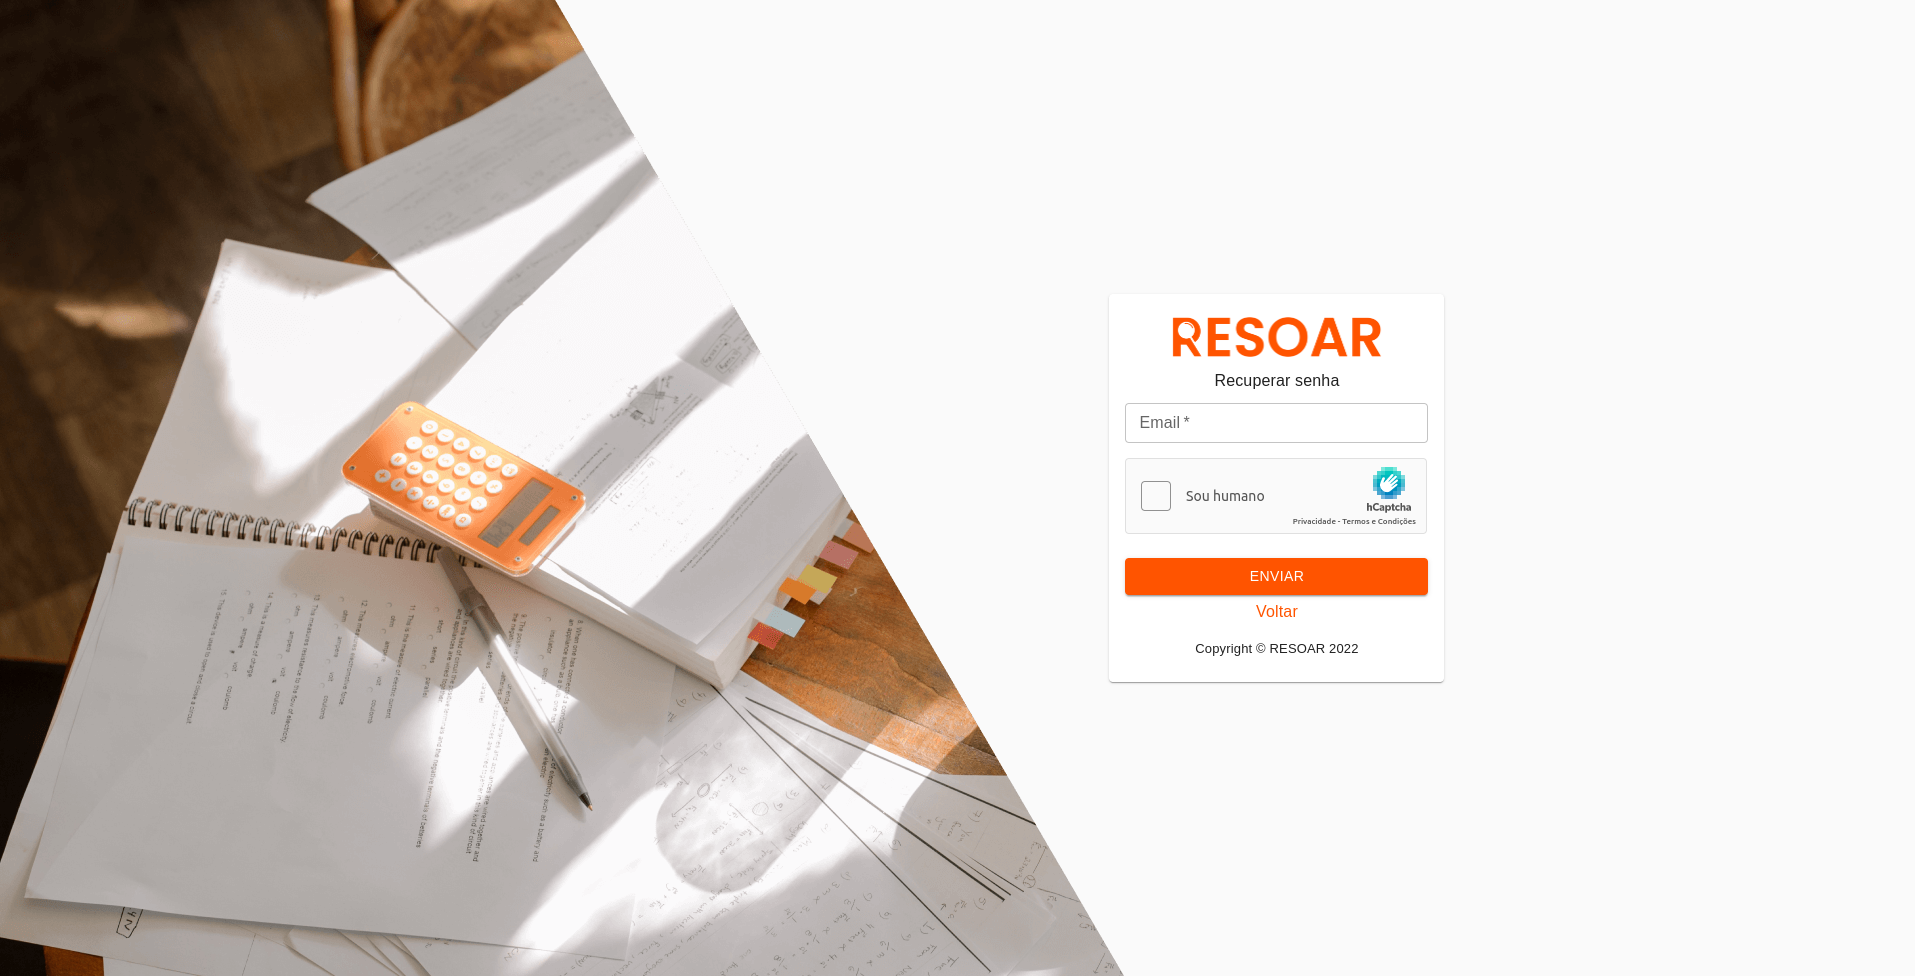
\includegraphics[scale=0.294]{img/resoar-password-recovery.png}}                                                                                                                                                                 \\ \hline
    \end{tabular}
\end{table}

\begin{table}[H]
    \caption{Visão geral}
    \begin{tabular}{|p{1cm}|p{14cm}|}
        \hline
        \multicolumn{1}{|c|}{\textbf{04}} & \textbf{Visão geral}                                                                                                                                                                                                                                                                            \\ \hline
        \multicolumn{2}{|l|}{\begin{tabular}[c]{@{}l@{}}\textbf{Como} usuário do sistema\\ \textbf{Eu quero} acessar uma tela de boas vindas ao entrar no sistema, contendo as\\ minhas publicações mais recentes, publicações salvas, e histórico de\\ publicações acessadas.\\ \textbf{Para que} tenha um ponto de partida.\end{tabular}} \\ \hline
        \multicolumn{2}{|l|}{\textbf{Critérios de aceitação}}                                                                                                                                                                                                                                                                               \\ \hline
        \multicolumn{2}{|l|}{\begin{tabular}[c]{@{}l@{}}1. Deve exibir ao menos as 3 ultimas publicações do usuário.\\2. Deve exibir ao menos as 3 ultimas publicações salvas para leitura.\\3. Deve exibir ao menos um histórico das 3 ultimas publicações acessadas. \end{tabular}}                                                       \\ \hline
        \multicolumn{2}{|c|}{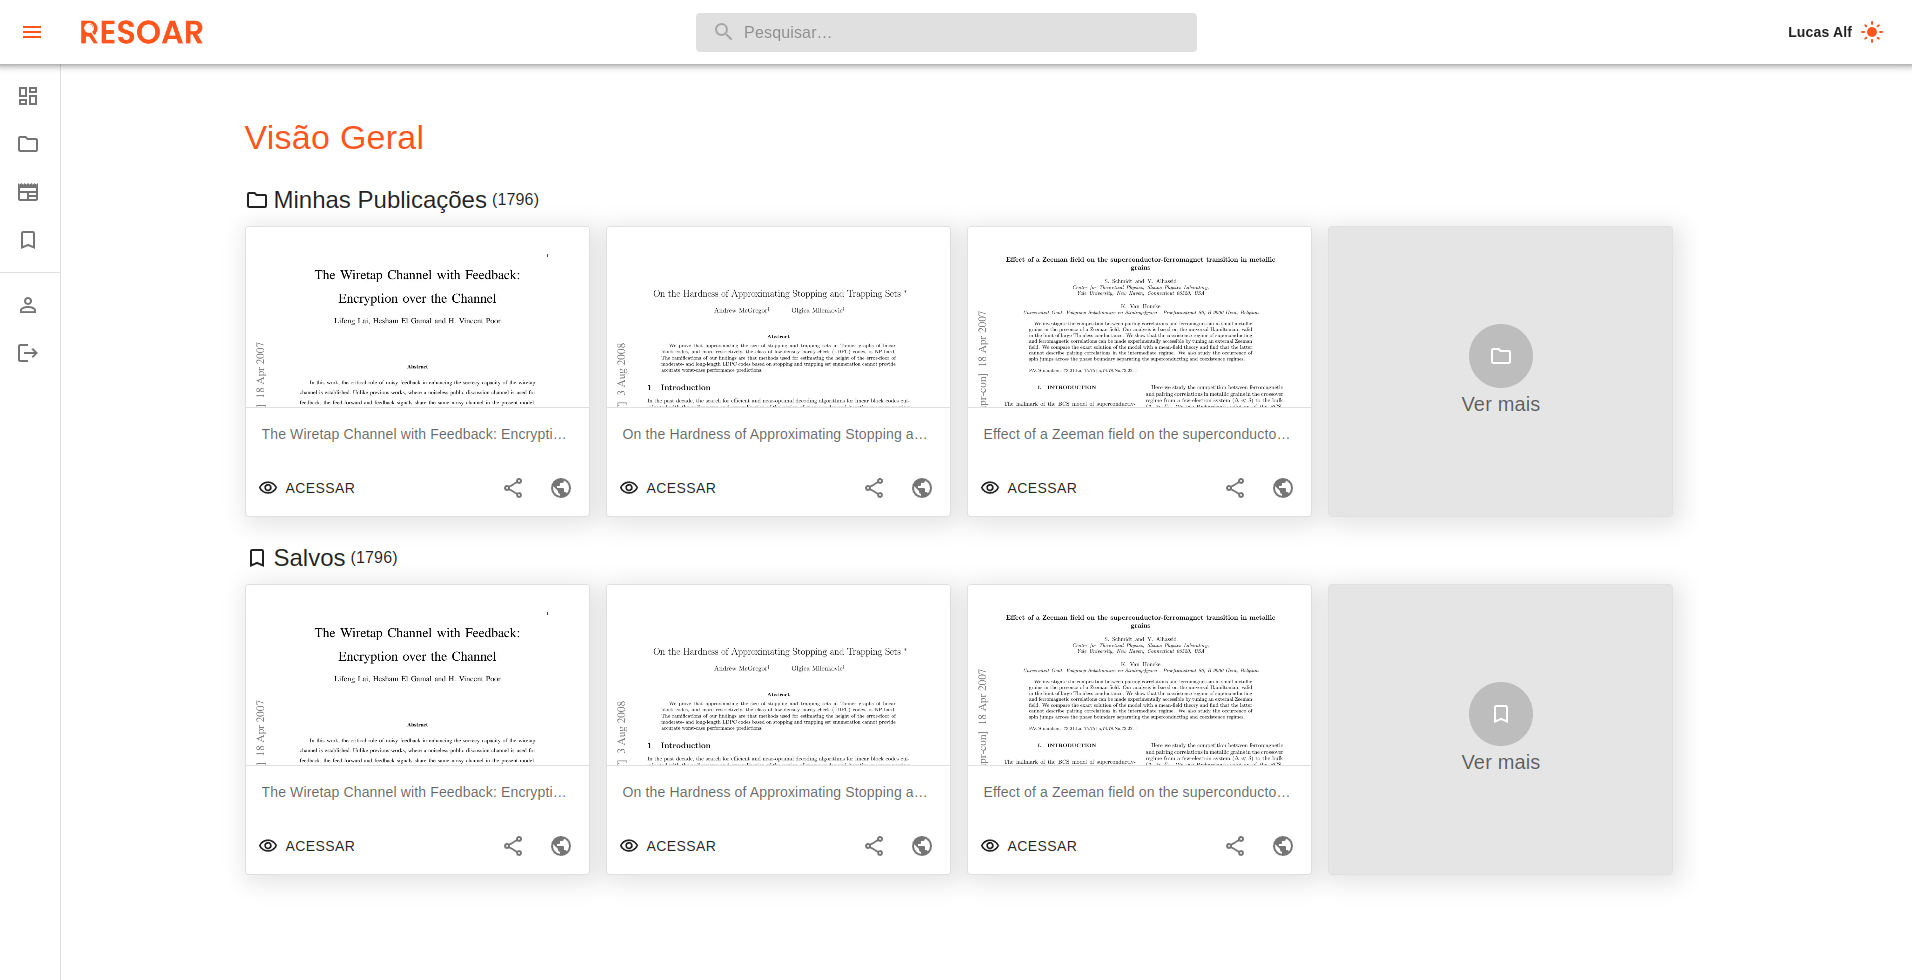
\includegraphics[scale=0.294]{img/resoar-overview.png}}                                                                                                                                                                                                                                                        \\ \hline
    \end{tabular}
\end{table}

\begin{table}[H]
    \caption{Minhas publicações}
    \begin{tabular}{|p{1cm}|p{14cm}|}
        \hline
        \multicolumn{1}{|c|}{\textbf{05}} & \textbf{Minhas publicações}                                                                                                                                                                                                                                                                                                                         \\ \hline
        \multicolumn{2}{|l|}{\begin{tabular}[c]{@{}l@{}}\textbf{Como} usuário do sistema\\ \textbf{Eu quero} acessar uma listagem contendo todas as minhas publicações\\ \textbf{Para que} possa navegar pelas publicações que realizei.\end{tabular}}                                                                                                                                          \\ \hline
        \multicolumn{2}{|l|}{\textbf{Critérios de aceitação}}                                                                                                                                                                                                                                                                                                                                   \\ \hline
        \multicolumn{2}{|l|}{\begin{tabular}[c]{@{}l@{}}1. Deve permitir a filtragem de publicações pelo título.\\2. Deve exibir na listagem o título, a imagem de capa, os autores, orientadores e\\ parte do resumo.\\3. Deve possuir um botão para a inclusão de nova publicação.\\4. Ao clicar em uma publicação, deve redirecionar para a página detalhada da\\ publicação. \end{tabular}} \\ \hline
        \multicolumn{2}{|c|}{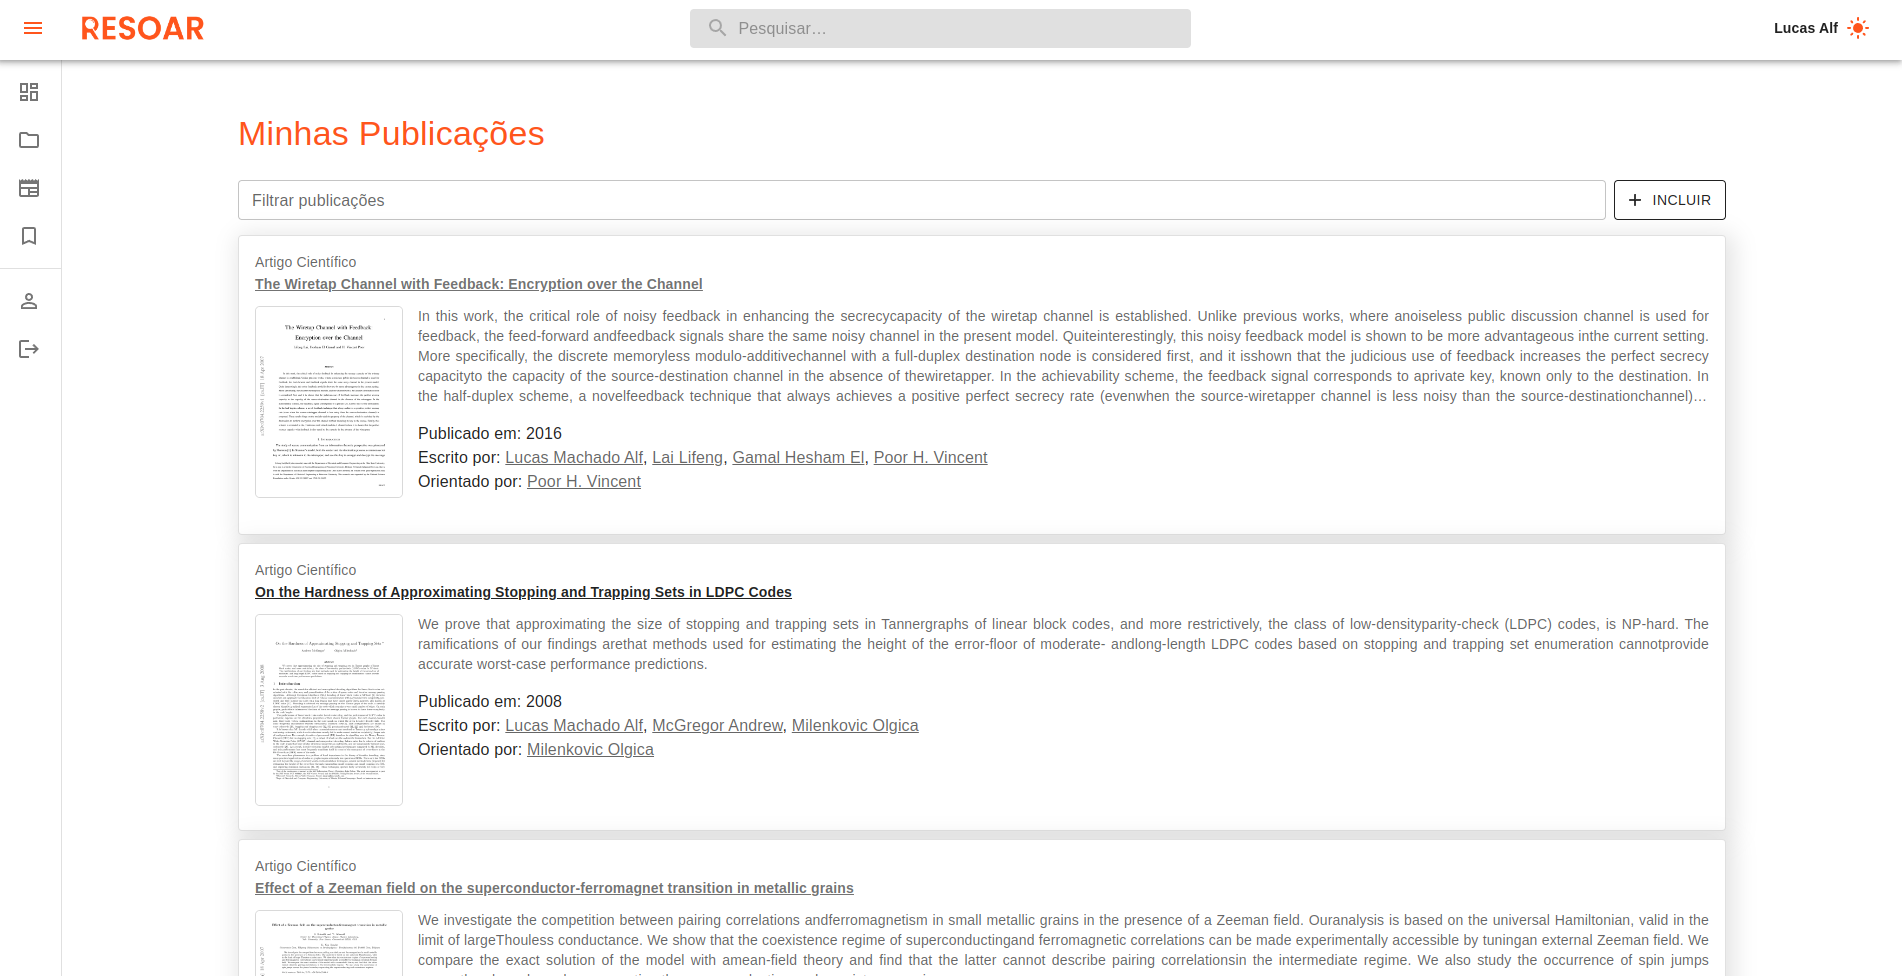
\includegraphics[scale=0.294]{img/resoar-my-research.png}}                                                                                                                                                                                                                                                                                                         \\ \hline
    \end{tabular}
\end{table}

\begin{table}[H]
    \caption{Nova publicação}
    \begin{tabular}{|p{1cm}|p{14cm}|}
        \hline
        \multicolumn{1}{|c|}{\textbf{06}} & \textbf{Nova publicação}                                                                                                                                                                                                                               \\ \hline
        \multicolumn{2}{|l|}{\begin{tabular}[c]{@{}l@{}}\textbf{Como} usuário do sistema\\ \textbf{Eu quero} realizar uma nova publicação\\ \textbf{Para que} possa salvar as minhas publicações no sistema.\end{tabular}}                                                                         \\ \hline
        \multicolumn{2}{|l|}{\textbf{Critérios de aceitação}}                                                                                                                                                                                                                                      \\ \hline
        \multicolumn{2}{|l|}{\begin{tabular}[c]{@{}l@{}}1. Deve solicitar os campos de título, resumo, ano, tipo, visibilidade, idioma,\\ instituição, autores, orientadores e arquivo da publicação.\\2. Dentro do campo de autores sempre deve haver no mínimo o próprio usuário. \end{tabular}} \\ \hline
        \multicolumn{2}{|c|}{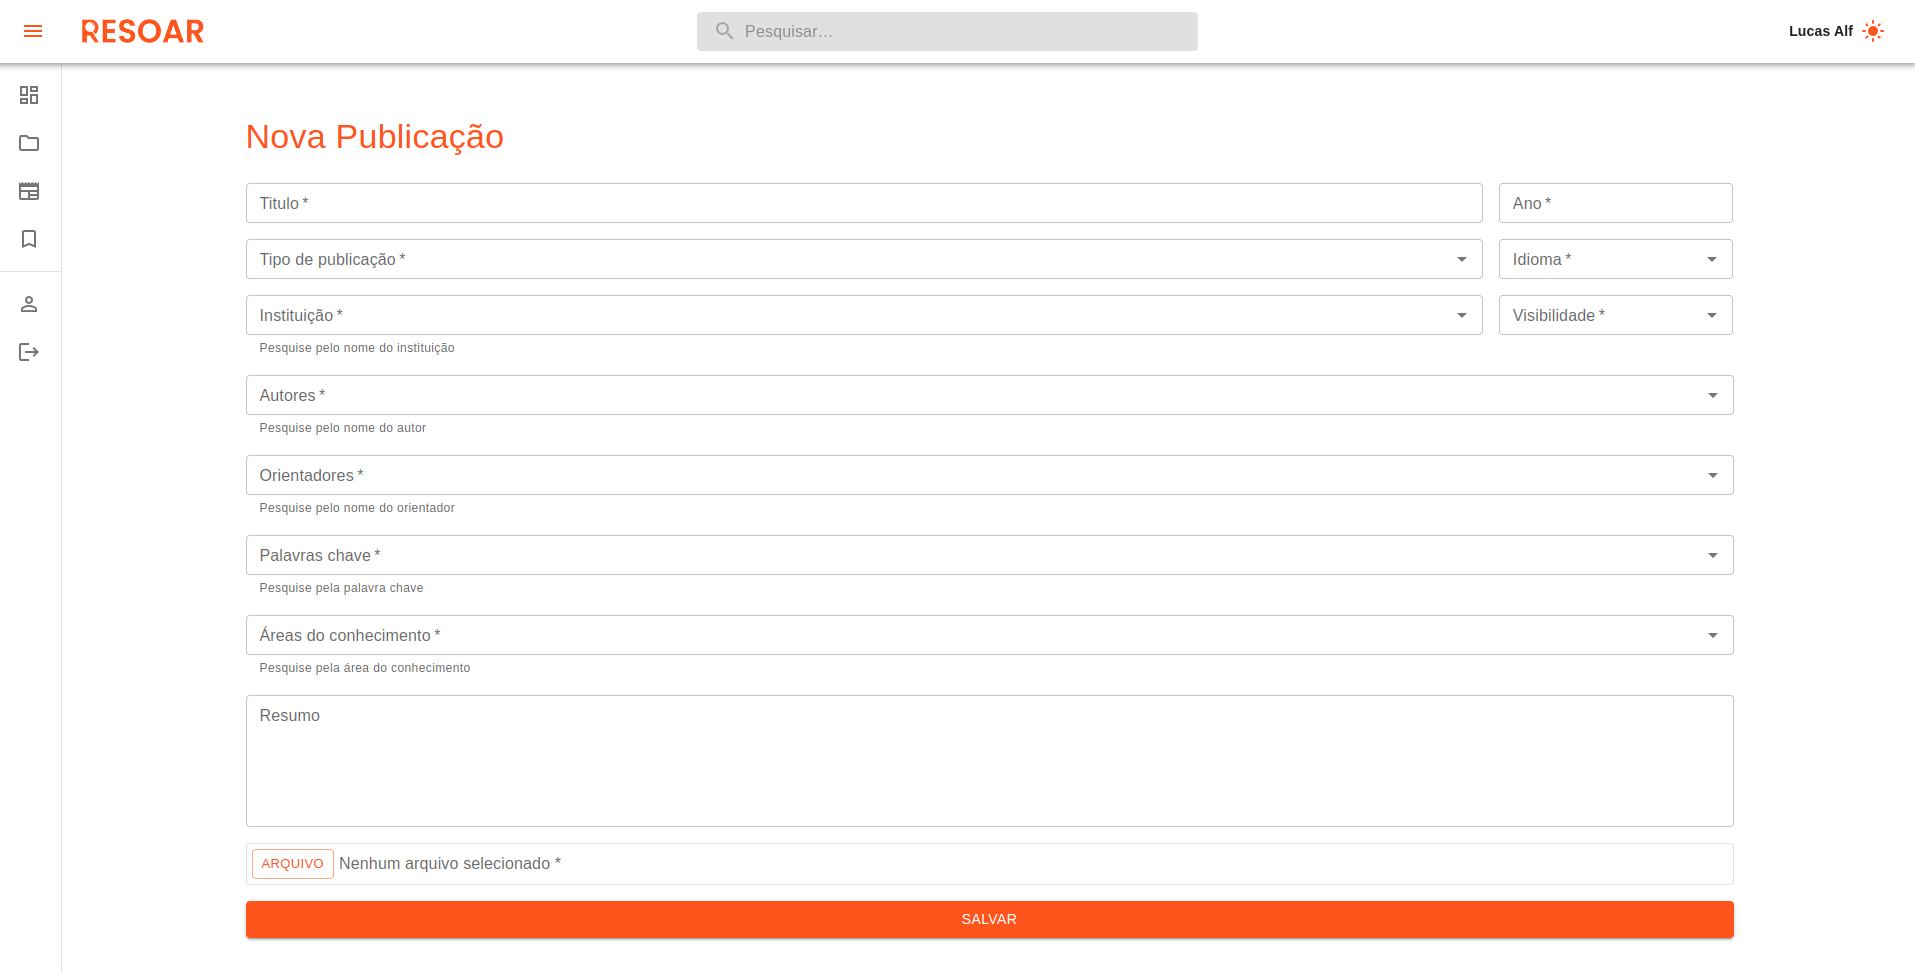
\includegraphics[scale=0.46]{img/resoar-add-research.png}}                                                                                                                                                                                                            \\ \hline
    \end{tabular}
\end{table}

\begin{table}[H]
    \caption{Pesquisar publicações}
    \begin{tabular}{|p{1cm}|p{14cm}|}
        \hline
        \multicolumn{1}{|c|}{\textbf{07}} & \textbf{Pesquisar publicações}                                                                                                                                                                                                                                           \\ \hline
        \multicolumn{2}{|l|}{\begin{tabular}[c]{@{}l@{}}\textbf{Como} usuário do sistema\\ \textbf{Eu quero} pesquisar por publicações, podendo utilizar de filtros \\ \textbf{Para que} possa encontrar as publicações que desejo visualizar.\end{tabular}}                                                         \\ \hline
        \multicolumn{2}{|l|}{\textbf{Critérios de aceitação}}                                                                                                                                                                                                                                                        \\ \hline
        \multicolumn{2}{|l|}{\begin{tabular}[c]{@{}l@{}}1. Deve permitir a busca por termos contidos dentro das publicações.\\2. Deve permitir a filtragem por ano, autor, orientador, tipo e idioma.\\3. Uma caixa de pesquisa por publicações sempre deve estar visível\\ na interface do usuário.  \end{tabular}} \\ \hline
        \multicolumn{2}{|c|}{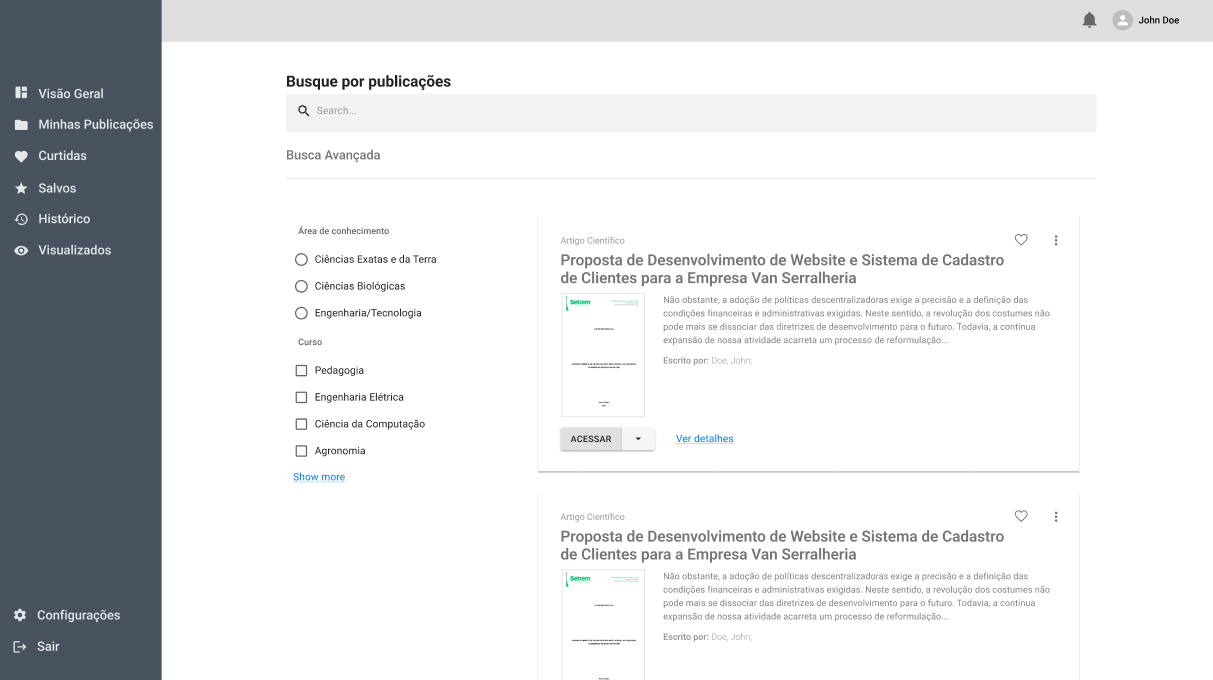
\includegraphics[scale=0.46]{img/resoar-search.png}}                                                                                                                                                                                                                                    \\ \hline
    \end{tabular}
\end{table}

\begin{table}[H]
    \caption{Visualizar publicação}
    \begin{tabular}{|p{1cm}|p{14cm}|}
        \hline
        \multicolumn{1}{|c|}{\textbf{08}} & \textbf{Visualizar publicação}                                                                                                                                                                                                                                                                                                                                                                       \\ \hline
        \multicolumn{2}{|l|}{\begin{tabular}[c]{@{}l@{}}\textbf{Como} usuário do sistema\\ \textbf{Eu quero} visualizar uma publicação \\ \textbf{Para que} possa ver os autores, orientadores, resumo e baixar o arquivo\\ da publicação.\end{tabular}}                                                                                                                                                                                         \\ \hline
        \multicolumn{2}{|l|}{\textbf{Critérios de aceitação}}                                                                                                                                                                                                                                                                                                                                                                                    \\ \hline
        \multicolumn{2}{|l|}{\begin{tabular}[c]{@{}l@{}}1. Deve exibir o título da publicação em destaque.\\2. Deve exibir a capa da publicação, e informações como os autores,\\ orientadores, tipo de publicação, idioma e resumo.\\3. Deve permitir realizar o \emph{download} da publicação.\\4. Deve permitir salvar a publicação para mais tarde.\\5. Deve permitir gerar um \emph{link} de compartilhamento da publicação. \end{tabular}} \\ \hline
        \multicolumn{2}{|c|}{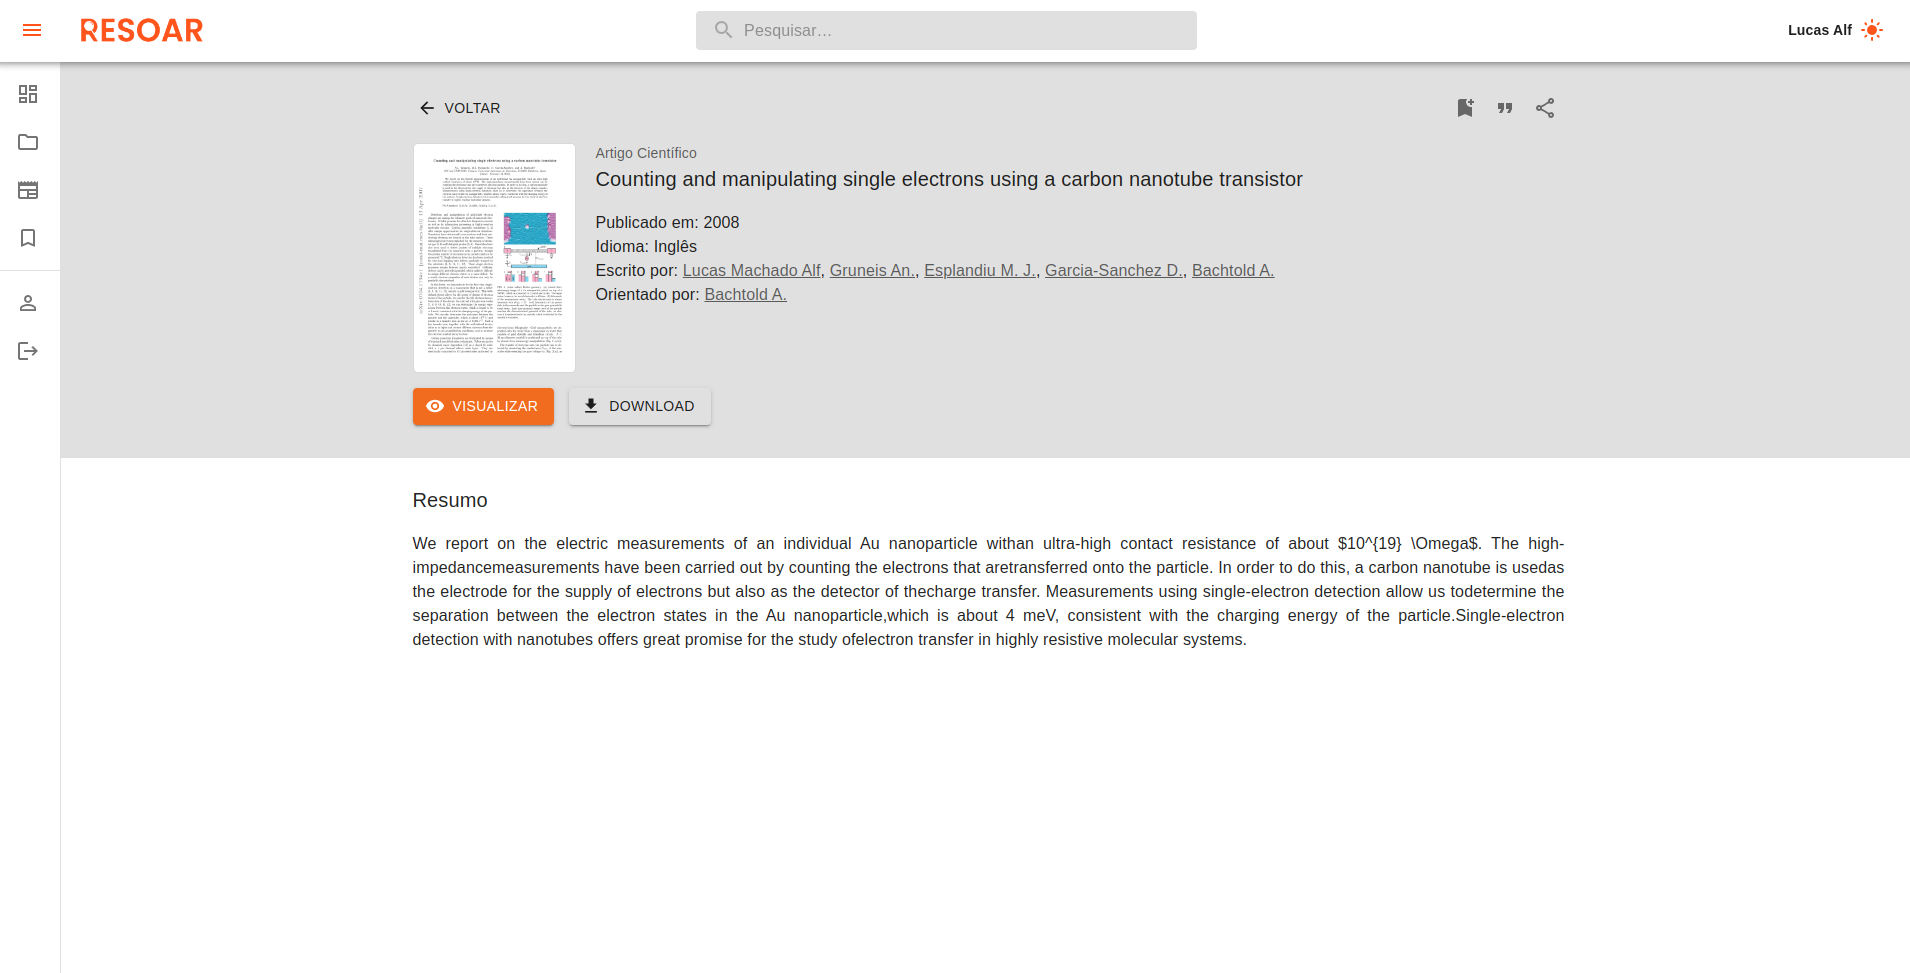
\includegraphics[scale=0.41]{img/resoar-view-research.png}}                                                                                                                                                                                                                                                                                                                                                         \\ \hline
    \end{tabular}
\end{table}

\begin{table}[H]
    \caption{Perfil do usuário}
    \begin{tabular}{|p{1cm}|p{14cm}|}
        \hline
        \multicolumn{1}{|c|}{\textbf{09}} & \textbf{Perfil do usuário}                                                                                                                                                                                                                                                  \\ \hline
        \multicolumn{2}{|l|}{\begin{tabular}[c]{@{}l@{}}\textbf{Como} usuário do sistema\\ \textbf{Eu quero} acessar uma página de perfil de usuário \\ \textbf{Para que} possa atualizar minhas informações, e trocar minha senha.\end{tabular}}                                                                       \\ \hline
        \multicolumn{2}{|l|}{\textbf{Critérios de aceitação}}                                                                                                                                                                                                                                                           \\ \hline
        \multicolumn{2}{|l|}{\begin{tabular}[c]{@{}l@{}}1. Deve exibir o nome e a foto do usuário.\\2. Deve listar as publicações as quais o usuário participa como autor.\\3. Caso o usuário esteja acessando o seu próprio perfil, devem existir opções\\ para editar as informações e trocar a senha. \end{tabular}} \\ \hline
        \multicolumn{2}{|c|}{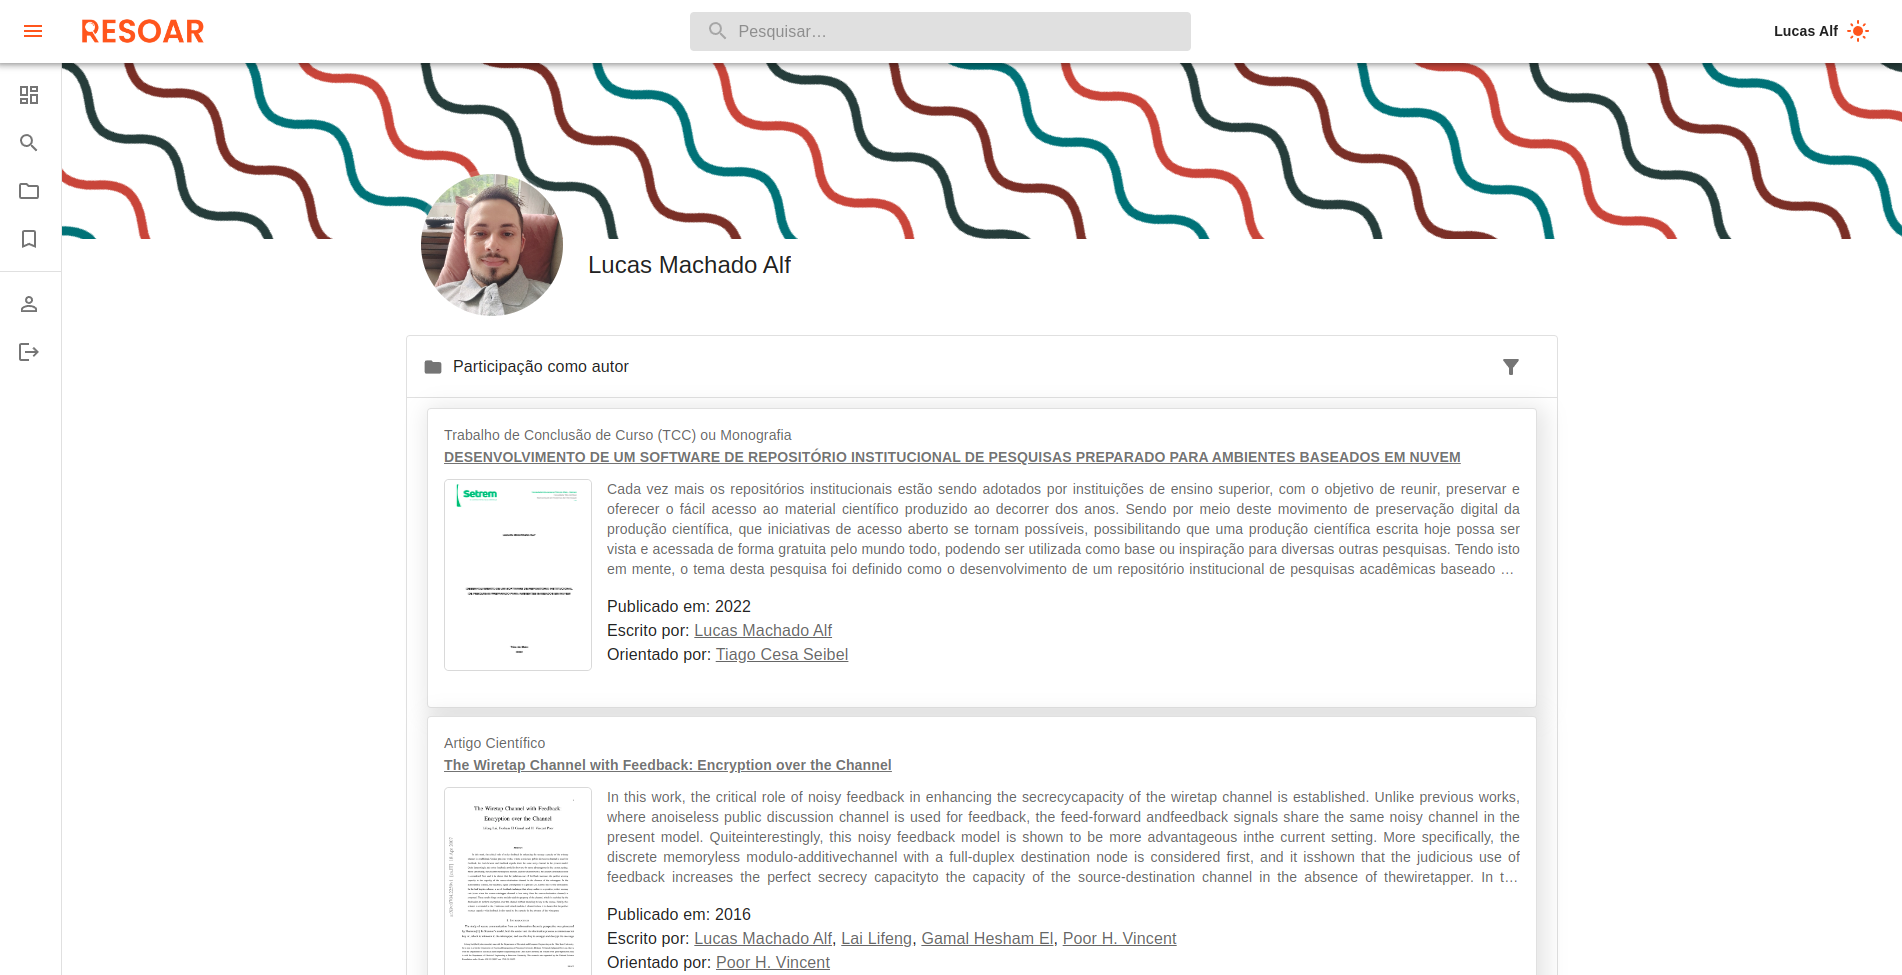
\includegraphics[scale=0.46]{img/resoar-account.png}}                                                                                                                                                                                                                                      \\ \hline
    \end{tabular}
\end{table}
